\documentclass[
  shownotes,
  xcolor={svgnames},
  hyperref={colorlinks,citecolor=DarkBlue,linkcolor=DarkRed,urlcolor=DarkBlue}
  ]{beamer}
\usepackage{animate}
\usepackage{amsmath}
\usepackage{amsfonts}
\usepackage{amssymb}
\usepackage{pifont}
\usepackage{mathpazo}
%\usepackage{xcolor}
\usepackage{multimedia}
\usepackage{fancybox}
\usepackage[para]{threeparttable}
\usepackage{multirow}
\setcounter{MaxMatrixCols}{30}
\usepackage{subcaption}
\usepackage{graphicx}
\usepackage{lscape}
\usepackage[compatibility=false,font=small]{caption}
\usepackage{booktabs}
\usepackage{ragged2e}
\usepackage{chronosys}
\usepackage{appendixnumberbeamer}
\usepackage{animate}
\setbeamertemplate{caption}[numbered]
\usepackage{color}
%\usepackage{times}
\usepackage{tikz}
\usepackage{comment} %to comment
%% BibTeX settings
\usepackage{natbib}
\bibliographystyle{apalike}
\bibpunct{(}{)}{,}{a}{,}{,}
\setbeamertemplate{bibliography item}{[\theenumiv]}

% Defines columns for bespoke tables
\usepackage{array}
\newcolumntype{L}[1]{>{\raggedright\let\newline\\\arraybackslash\hspace{0pt}}m{#1}}
\newcolumntype{C}[1]{>{\centering\let\newline\\\arraybackslash\hspace{0pt}}m{#1}}
\newcolumntype{R}[1]{>{\raggedleft\let\newline\\\arraybackslash\hspace{0pt}}m{#1}}


\usepackage{xfrac}


\usepackage{multicol}
\setlength{\columnsep}{0.5cm}

% Theme and colors
\usetheme{Boadilla}

% I use steel blue and a custom color palette. This defines it.
\definecolor{andesred}{HTML}{af2433}

% Other options
\providecommand{\U}[1]{\protect\rule{.1in}{.1in}}
\usefonttheme{serif}
\setbeamertemplate{itemize items}[default]
\setbeamertemplate{enumerate items}[square]
\setbeamertemplate{section in toc}[circle]

\makeatletter

\definecolor{mybackground}{HTML}{82CAFA}
\definecolor{myforeground}{HTML}{0000A0}

\setbeamercolor{normal text}{fg=black,bg=white}
\setbeamercolor{alerted text}{fg=red}
\setbeamercolor{example text}{fg=black}

\setbeamercolor{background canvas}{fg=myforeground, bg=white}
\setbeamercolor{background}{fg=myforeground, bg=mybackground}

\setbeamercolor{palette primary}{fg=black, bg=gray!30!white}
\setbeamercolor{palette secondary}{fg=black, bg=gray!20!white}
\setbeamercolor{palette tertiary}{fg=white, bg=andesred}

\setbeamercolor{frametitle}{fg=andesred}
\setbeamercolor{title}{fg=andesred}
\setbeamercolor{block title}{fg=andesred}
\setbeamercolor{itemize item}{fg=andesred}
\setbeamercolor{itemize subitem}{fg=andesred}
\setbeamercolor{itemize subsubitem}{fg=andesred}
\setbeamercolor{enumerate item}{fg=andesred}
\setbeamercolor{item projected}{bg=gray!30!white,fg=andesred}
\setbeamercolor{enumerate subitem}{fg=andesred}
\setbeamercolor{section number projected}{bg=gray!30!white,fg=andesred}
\setbeamercolor{section in toc}{fg=andesred}
\setbeamercolor{caption name}{fg=andesred}
\setbeamercolor{button}{bg=gray!30!white,fg=andesred}


\usepackage{fancyvrb}
\newcommand{\VerbBar}{|}
\newcommand{\VERB}{\Verb[commandchars=\\\{\}]}
\DefineVerbatimEnvironment{Highlighting}{Verbatim}{commandchars=\\\{\}}
% Add ',fontsize=\small' for more characters per line
\usepackage{framed}
\definecolor{shadecolor}{RGB}{248,248,248}
\newenvironment{Shaded}{\begin{snugshade}}{\end{snugshade}}
\newcommand{\AlertTok}[1]{\textcolor[rgb]{0.94,0.16,0.16}{#1}}
\newcommand{\AnnotationTok}[1]{\textcolor[rgb]{0.56,0.35,0.01}{\textbf{\textit{#1}}}}
\newcommand{\AttributeTok}[1]{\textcolor[rgb]{0.77,0.63,0.00}{#1}}
\newcommand{\BaseNTok}[1]{\textcolor[rgb]{0.00,0.00,0.81}{#1}}
\newcommand{\BuiltInTok}[1]{#1}
\newcommand{\CharTok}[1]{\textcolor[rgb]{0.31,0.60,0.02}{#1}}
\newcommand{\CommentTok}[1]{\textcolor[rgb]{0.56,0.35,0.01}{\textit{#1}}}
\newcommand{\CommentVarTok}[1]{\textcolor[rgb]{0.56,0.35,0.01}{\textbf{\textit{#1}}}}
\newcommand{\ConstantTok}[1]{\textcolor[rgb]{0.00,0.00,0.00}{#1}}
\newcommand{\ControlFlowTok}[1]{\textcolor[rgb]{0.13,0.29,0.53}{\textbf{#1}}}
\newcommand{\DataTypeTok}[1]{\textcolor[rgb]{0.13,0.29,0.53}{#1}}
\newcommand{\DecValTok}[1]{\textcolor[rgb]{0.00,0.00,0.81}{#1}}
\newcommand{\DocumentationTok}[1]{\textcolor[rgb]{0.56,0.35,0.01}{\textbf{\textit{#1}}}}
\newcommand{\ErrorTok}[1]{\textcolor[rgb]{0.64,0.00,0.00}{\textbf{#1}}}
\newcommand{\ExtensionTok}[1]{#1}
\newcommand{\FloatTok}[1]{\textcolor[rgb]{0.00,0.00,0.81}{#1}}
\newcommand{\FunctionTok}[1]{\textcolor[rgb]{0.00,0.00,0.00}{#1}}
\newcommand{\ImportTok}[1]{#1}
\newcommand{\InformationTok}[1]{\textcolor[rgb]{0.56,0.35,0.01}{\textbf{\textit{#1}}}}
\newcommand{\KeywordTok}[1]{\textcolor[rgb]{0.13,0.29,0.53}{\textbf{#1}}}
\newcommand{\NormalTok}[1]{#1}
\newcommand{\OperatorTok}[1]{\textcolor[rgb]{0.81,0.36,0.00}{\textbf{#1}}}
\newcommand{\OtherTok}[1]{\textcolor[rgb]{0.56,0.35,0.01}{#1}}
\newcommand{\PreprocessorTok}[1]{\textcolor[rgb]{0.56,0.35,0.01}{\textit{#1}}}
\newcommand{\RegionMarkerTok}[1]{#1}
\newcommand{\SpecialCharTok}[1]{\textcolor[rgb]{0.00,0.00,0.00}{#1}}
\newcommand{\SpecialStringTok}[1]{\textcolor[rgb]{0.31,0.60,0.02}{#1}}
\newcommand{\StringTok}[1]{\textcolor[rgb]{0.31,0.60,0.02}{#1}}
\newcommand{\VariableTok}[1]{\textcolor[rgb]{0.00,0.00,0.00}{#1}}
\newcommand{\VerbatimStringTok}[1]{\textcolor[rgb]{0.31,0.60,0.02}{#1}}
\newcommand{\WarningTok}[1]{\textcolor[rgb]{0.56,0.35,0.01}{\textbf{\textit{#1}}}}
\usepackage{graphicx}
\makeatletter

\makeatother






%%%%%%%%%%%%%%% BEGINS DOCUMENT %%%%%%%%%%%%%%%%%%

\begin{document}

\title[Lecture 3]{Lecture 3: \\ OLS \& Prediction in/out of Sample}
\subtitle{Big Data and Machine Learning for Applied Economics \\ Econ 4676}
\date{\today}

\author[Sarmiento-Barbieri]{Ignacio Sarmiento-Barbieri}
\institute[Uniandes]{Universidad de los Andes}


\begin{frame}[noframenumbering]
\maketitle
\end{frame}

%%%%%%%%%%%%%%%%%%%%%%%%%%%%%%%%%%%
%       Motivation              %
% What is the question?
% Why do we care?
% What is new?
% What do you find?
%%%%%%%%%%%%%%%%%%%%%%%%%%%%%%%%%%%




\begin{frame}
\frametitle{Agenda}

\tableofcontents


\end{frame}



%%----------------------------------------------------------------------%
\section{Recap}
%----------------------------------------------------------------------%

\begin{frame}
\frametitle{Recap}

\begin{itemize} 
    \item We started shifting paradigms
    \bigskip
    \item Decision Theory: Risk with square error loss $\rightarrow$ MSE
    \bigskip
    \item Objective minimize the reducible error
    \bigskip
    \item Irreducible error our unknown bound
    \bigskip
    \item Machine Learning best kept secret:  some bias can help lower MSE
\end{itemize}
\end{frame}

%----------------------------------------------------------------------%
\section{Motivation}
%----------------------------------------------------------------------%
\begin{frame}
\frametitle{Motivation}

\begin{itemize}
  \item Linear regression is the “work horse” of econometrics and (supervised) machine learning. 
  \bigskip
  \item Very powerful in many contexts:
  \bigskip
  \begin{itemize}
    \item Model Spatial Relationships
    \item Non linear relationships
  \end{itemize}
  \bigskip
  \item It can be used also for classification. 
  \bigskip
  \item Big `payday' to study this model in detail.
\end{itemize}
\end{frame}

%----------------------------------------------------------------------%
\section{Linear Regression}
%----------------------------------------------------------------------%

\begin{frame}
\frametitle{Linear Regression Model}

{\bf Problem}

%We have a set of inputs $X$ and want to predict a real valued output $y$

\begin{figure}[H] \centering
  \centering
  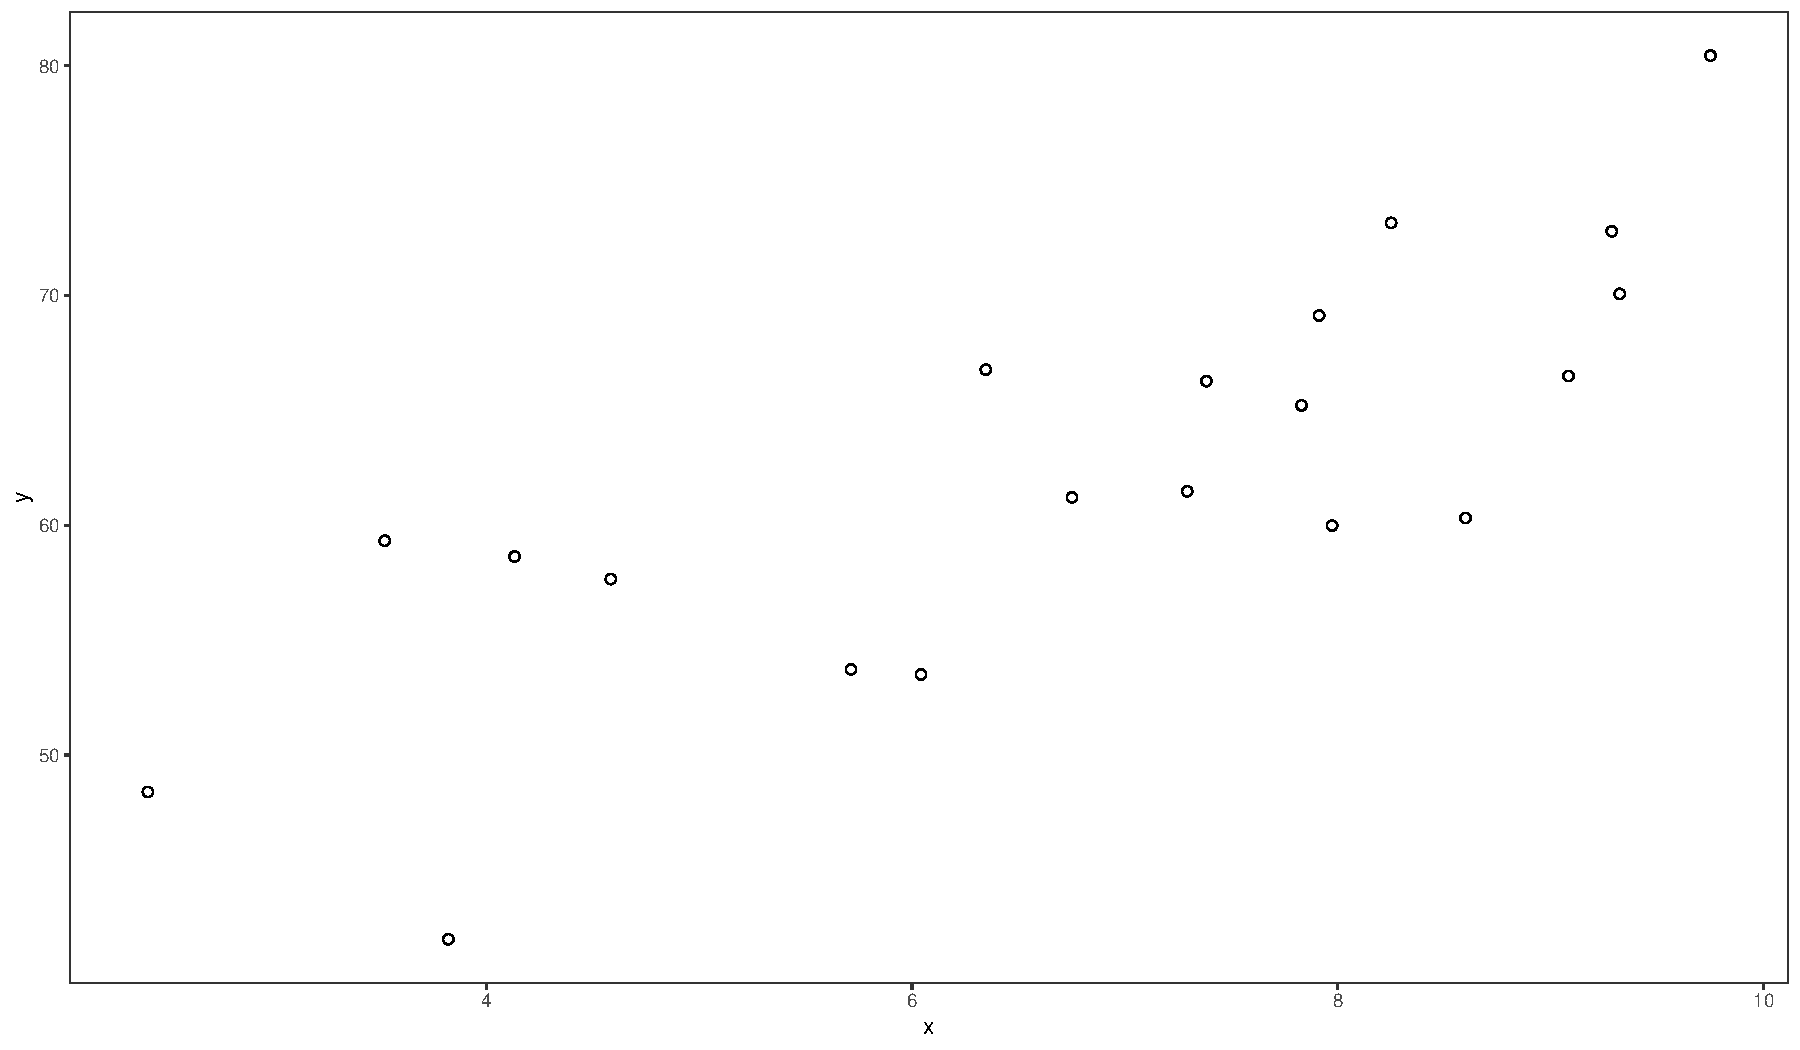
\includegraphics[scale=0.25]{figures/fig_1.pdf}
  \\
  \tiny
\end{figure}


\end{frame}
%----------------------------------------------------------------------%
\begin{frame}
\frametitle{Linear Regression Model}
\bigskip
$f(X)=X\beta$ and the interest is on estimating $\beta$
\begin{align}
y = X \beta +u
\end{align}

where 
\begin{itemize}
  \item y is a vector $n \times 1$ with typical element $y_i$
  \item X is a matrix $n \times k$ 
  \begin{itemize}
    \tiny
      \item Note that we can represent it as a column vector $\underset{n\times k}{X}=[\underset{n\times 1}{X_1}\,\,\underset{n\times 1}{X_2}\dots \underset{n\times 1}{X_k}] $
  \end{itemize}
  \item $\beta$ is a vector $k \times 1$ with typical element $\beta_j$
\end{itemize}

\bigskip
Thus 

\begin{align}
y_i &= X_i' \beta +u_i  \\ \nonumber
    &= \sum_{j=1}^k \beta_j X_{ji} +u_i
\end{align}

\end{frame}

%----------------------------------------------------------------------%
\begin{frame}
\frametitle{Linear Regression Model}

How do we estimate $\beta$?

\begin{itemize}
  \footnotesize
  \item Method of Moments {\tiny (for HW)}
  \item MLE {\tiny (more on this later)}
  \item OLS: minimize risk squared error loss $\rightarrow$ minimizes RSS ($e'e$) 
  \begin{itemize}
    \tiny
  \item where $e=Y-\hat Y=Y-X\hat\beta$
  \item In the HW, you will show that min RSS same as max $R^2$
  \end{itemize}  
\end{itemize}
\bigskip

OLS solution: $\hat \beta = (X'X)^{-1} X'y$

\bigskip
\begin{figure}[H] \centering
  \centering
  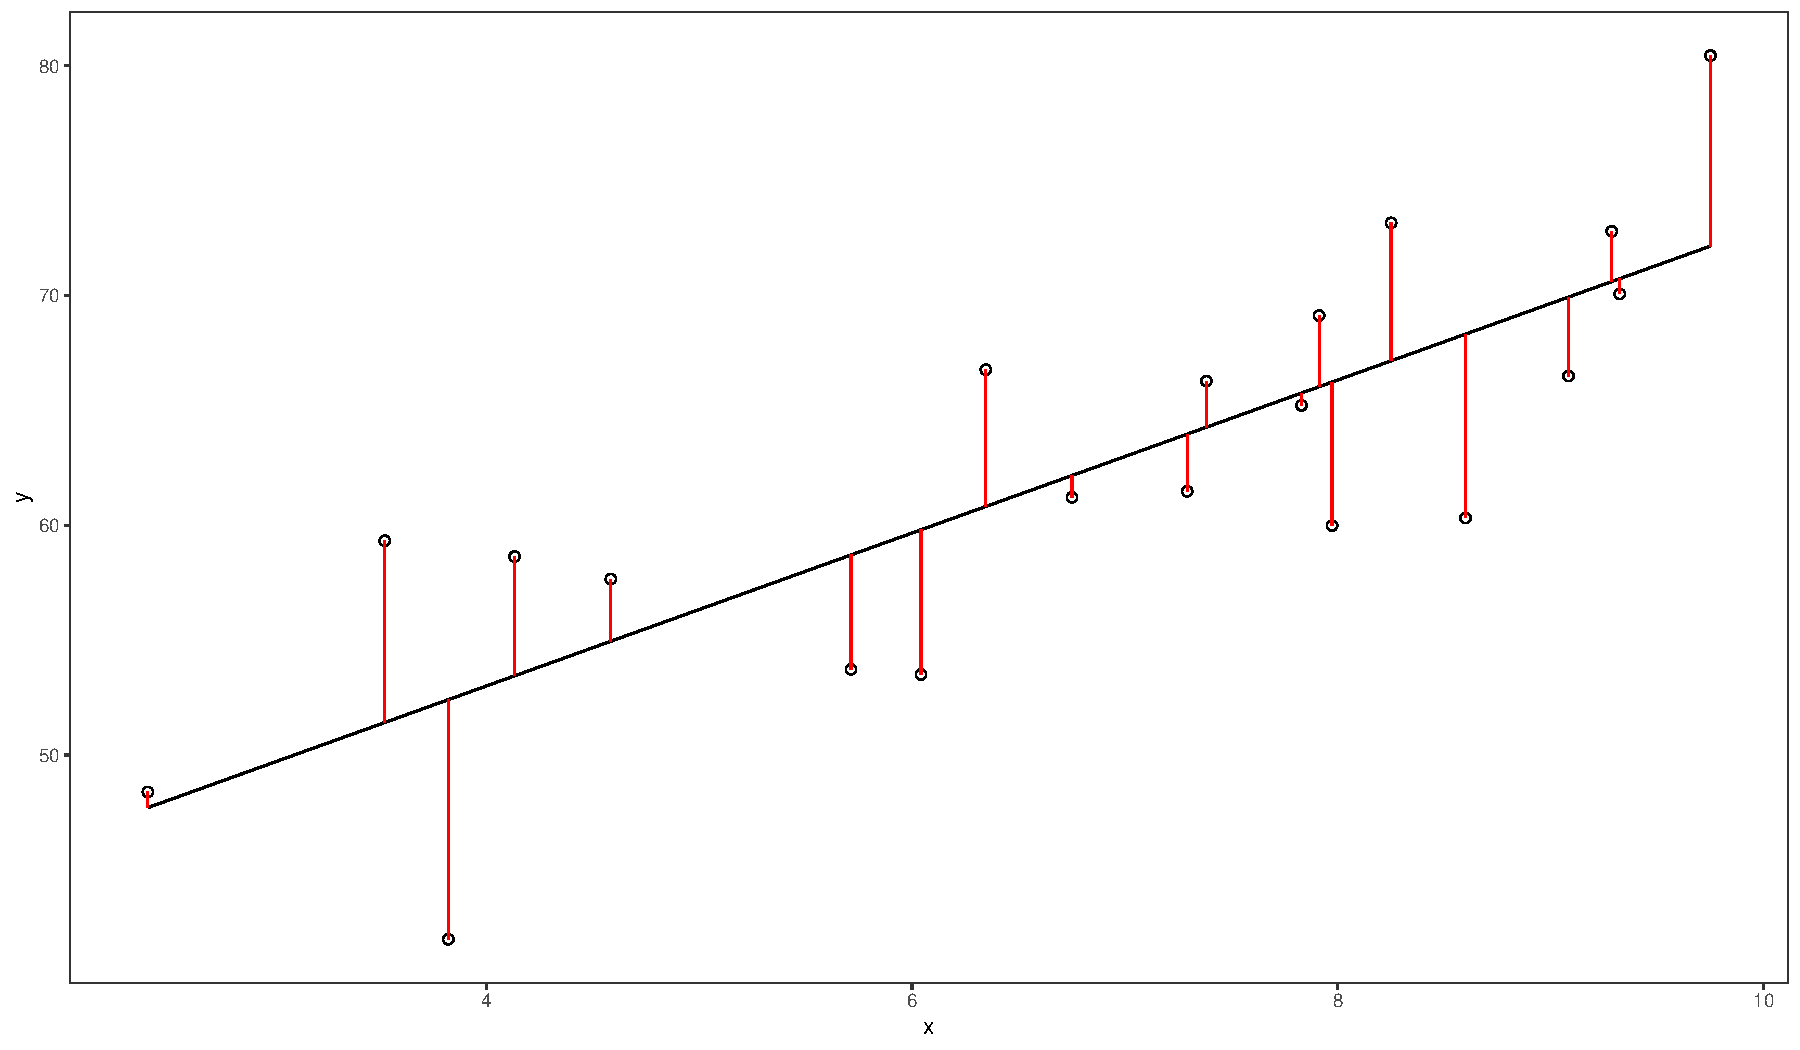
\includegraphics[scale=0.22]{figures/fig_1b.pdf}
  \\
  \tiny
\end{figure}


\end{frame}
%----------------------------------------------------------------------%
\begin{frame}
\frametitle{Gauss Markov Theorem}


Gauss-Markov Theorem says that 
\bigskip
\begin{align}
 \hat \beta = (X'X)^{-1} X'y
\end{align}

\bigskip

\begin{itemize}
  \item The OLS estimator ($\hat \beta$) is BLUE, the more efficient than any other linear unbiased estimator, 
  \medskip
  \item Efficiency in the sense that  $Var(\tilde \beta) - Var(\hat \beta)$ is positive semidefinite matrix.
\end{itemize}

\bigskip
\tiny Proof: HW. Tip: a matrix $M_{p\times p}$ is positive semi-definite iff $c'Mc\geq0$ $\forall x\in \mathbb{R}^p$

\end{frame}


%----------------------------------------------------------------------%
\begin{frame}
\frametitle{Gauss Markov Theorem}

\begin{itemize}
  \item Gauss Markov Theorem that says OLS is BLUE is perhaps one of the most famous results in statistics. 
  
  \begin{itemize}
    \item $E(\hat\beta) = \beta$
    \medskip 
    \item $V(\hat \beta ) = \sigma^2 (X'X)^{-1}$
  \end{itemize}
  
\bigskip
  \item However, it is essential to note the limitations of the theorem. 

  \begin{itemize}
    \footnotesize
    \item Correctly specified with exogenous Xs, 
      \medskip 
    \item The term error is homoscedastic 
      \medskip 
    \item No serial correlation.
      \medskip 
    \item Nothing about the OLS estimator being the more efficient than any other estimator one can imagine.
  \end{itemize}
    
    %\medskip 
    %\item Estimators that are nonlinear and/or biased may have a better performance than OLS 
  

\end{itemize}

\end{frame}


%----------------------------------------------------------------------%
\begin{frame}
\frametitle{Prediction vs Estimation}

\begin{itemize}
\item {\bf Predicting well means estimating well}

  \bigskip 
\begin{itemize}
  \item Note that the prediction of $y$ will be given by $\hat y=X \hat \beta$
  \bigskip 
  \item Under Gauss-Markov framework
  
  \begin{itemize}
    \item $E(\hat y) = X\beta$
    \medskip 
    \item $V(\hat y ) = \sigma^2 X' (X'X)^{-1} X$
  \end{itemize}
\end{itemize}

  \bigskip 

\item Then if $\hat \beta$ is unbiased and of minimum variance, 
\item then $\hat y$ is an unbiased predictor and minimum variance, from the class of unbiased linear estimators/predictors
  \begin{itemize}
    \tiny 
    \item Proof: for HW similar to $\hat \beta$ proof
  \end{itemize}
\end{itemize}
\end{frame}

\subsection{Prediction vs Estimation}
%----------------------------------------------------------------------%
\begin{frame}
\frametitle{Prediction vs Estimation}

\begin{itemize}
\item {\bf Estimation Accuracy}

\begin{align}
  MSE(\beta) &= E(\hat \beta - \beta) \\
             &= E(\beta - E(\hat \beta))^2 + Var(\hat \beta) 
\end{align}

\item  Intuitively, the result says that how wrong is the estimate (MSE) depends on: 
\bigskip
  \begin{itemize}
  \item how uncentered it is (bias) and 
  \item how dispersed it is around its center (variance). 
  \end{itemize}
\end{itemize}

\end{frame}

\subsection{Prediction vs Predictive Error}
%----------------------------------------------------------------------%
\begin{frame}
\frametitle{Prediction and Predictive Error}

\begin{itemize}
  \item Now suppose that the goal is to predict $Y$ with another random variable $\hat Y$.
  \bigskip
  \item The \emph{prediction error} is defined as:
\end{itemize}
  \bigskip

  \begin{align}
    Err(\hat Y) \equiv E\left(Y-\hat Y\right)^2\
  \end{align}

\begin{itemize}
  \item Conceptually the prediction error is equal to the MSE
  \bigskip
  \item However, MSE compares a RV ($\hat \beta$) with a parameter ($\beta$)
  \bigskip
  \item $Err(\hat Y)$ involves two RV 
\end{itemize}



\end{frame}

%----------------------------------------------------------------------%
\begin{frame}
\frametitle{Prediction and predictive error}

\begin{itemize}
  \item More concretely, the goal is to predict $Y$ given another variable $X$. 
  \bigskip
  \item We  assume that the link between $Y$ and $X$ is given by the simple model:
\end{itemize}
\bigskip
\begin{align}
  Y = f(X) + u
\end{align}
\bigskip
\begin{itemize}
  \item where $f(X)$ is any function, 
  \bigskip
  \item  $u$ is an unobserved random variable with $E(u)=0$ and $V(u) = \sigma^2$
\end{itemize}


\end{frame}

%----------------------------------------------------------------------%
\begin{frame}
\frametitle{Prediction and predictive error}

\begin{itemize}
  \item In practice we don't observe $f(X)$
  \item We need to estimate it with $\hat f(X)$ a RV 

\end{itemize}

\bigskip
Then 
\begin{align}
  Err (\hat Y )  &= MSE(\hat f) + \sigma^2  \\
                 &= Bias^2(\hat f) + V(\hat f) + \sigma^2
\end{align}
\bigskip
Two parts:
\begin{itemize}
  \item  the error from estimating $f$ with $\hat f$. (\emph{reducible})
  \item  the error from not being able to observe $u$. (\emph{irreducible})
\end{itemize}

\bigskip

This is an important result, predicting $Y$ properly we need a good estimate of $f$.

\end{frame}


%----------------------------------------------------------------------%
\begin{frame}
\frametitle{Prediction and Linear regression}

\begin{itemize}
  \item Linear regression sets 
\end{itemize}
\bigskip
\begin{equation}\label{eq:3_1_7}
f(X)= \beta_1 +\beta_2 X_2 +\dots+\beta_k X_k
\end{equation}

\bigskip
\begin{itemize}
  \item In classical econometrics this model is given
  \item Focus is on the estimation of the unknown parameters $\beta_1,\dots,\beta_k$. 
  \item The prediction for $Y$ is given by:
\end{itemize}

\begin{equation}\label{eq:3_1_8}
\hat{Y} = \hat{\beta}_1 + \hat{\beta}_2 X_2 + \dots + \hat{\beta}_k X_k
\end{equation}

\bigskip
\begin{itemize}
  \item where $\hat{\beta}_1,\dots,\hat{\beta}_k$ are estimates. 
\end{itemize}


\end{frame}
%----------------------------------------------------------------------%
\begin{frame}
\frametitle{Prediction and linear regression}

\begin{itemize}
  \item Under the classical assumptions the OLS estimator is unbiased, hence 
\end{itemize}

\begin{align}
  E(\hat f)&= E(\hat{\beta}_1 + \hat{\beta}_2 X_2 + \dots + \hat{\beta}_k X_k) \\ 
  &= E(\hat{\beta}_1) + E(\hat{\beta}_2) X_2 + \dots + E(\hat{\beta}_k) X_k  \\ 
  &= f
\end{align}




Then, 

\begin{itemize}
  \item $MSE(\hat f)$ reduces to just $V(\hat f)$
\end{itemize} 


\end{frame}

%----------------------------------------------------------------------%
\begin{frame}
\frametitle{Complexity and the variance/bias trade off}

\begin{itemize}

  \item When the focus switches from estimating $f$ to predicting $Y$, 
  \bigskip
  \item $f$ plays a secondary role, as just a tool to improve the prediction based on $X$.
  \bigskip
  \item  Predicting $Y$ involves \emph{learning} $f$, that is, $f$ is no longer taken as given, as in the classical view. 
  \bigskip
  \item Now it implies an iterative process where initial choices for $f$ are revised in light of potential improvements in predictive performance.
  \bigskip
  \item Model choice or learning involves choosing both $f$ and a strategy to estimate it ($\hat f$), guided by predictive performance. 

\end{itemize}


\end{frame}

%----------------------------------------------------------------------%
\begin{frame}
\frametitle{Complexity and the variance/bias trade off}

\begin{itemize}
\item Classical econometrics, model choice involves deciding between a smaller and a larger linear model. 
\item Consider the following competing models for $y$:

\end{itemize}
\bigskip
\begin{equation}
Y=\beta_1 X_1 + u_1
\end{equation}

and

\begin{equation}
Y=\beta_1 X_1 + \beta_2 X_2 + u_2
\end{equation}

\bigskip
\begin{itemize}
  \item $\hat \beta^{(1)}_1$ the OLS estimator of regressing $y$ on $X_1$
  \item  $\hat \beta^{(2)}_1$ and $\hat \beta^{(2)}_2$ the OLS estimators of $\beta_1$ and $\beta_2$ of regressing $Y$ on $X_1$ and $X_2$. 
\end{itemize}
 
\end{frame}

%----------------------------------------------------------------------%
\begin{frame}
\frametitle{Complexity and the variance/bias trade off}

The corresponding predictions will be

\begin{equation}\label{eq:3_2_3}
\hat{Y}^{(1)}=\hat{\beta}^{(1)}_1 X_1 
\end{equation}

and

\begin{equation}\label{eq:3_2_4}
\hat{Y}^{(2)}=\hat{\beta}^{(2)}_1 X_1 + \hat{\beta}^{(2)}_2 X_2 
\end{equation}

\end{frame}

%----------------------------------------------------------------------%
\begin{frame}
\frametitle{Complexity and the variance/bias trade off}

\begin{itemize}
  \item An important discussion in classical econometrics is that of omission of relevant variables vs. inclusion of irrelevant ones. 
  \begin{itemize}
    \item If model (1) is true then estimating the larger model (2) leads to inefficient though unbiased estimators due to unnecessarily including $X_2$. 
    \item If model (2) holds, estimating the smaller model (1) leads to a more efficient but biased estimate if $X_1$ is also correlated with the omitted regressor $X_2$. 
  \end{itemize}
  \bigskip
  \item This discussion of small vs large is always with respect to a model that is supposed to be true.
  \bigskip
\item  But in practice the true model is unknown. 
\bigskip
\end{itemize}


\end{frame}

%----------------------------------------------------------------------%
\begin{frame}
\frametitle{Complexity and the variance/bias trade off}


\begin{itemize}
  \item Choosing between models involves a {\it bias/variance trade off}
  \medskip
\item Classical econometrics tends to solve this dilemma abruptly, 
  \begin{itemize}
    \item  requiring unbiased estimation, and hence favoring larger models to avoid bias
  \end{itemize}
\medskip
\item In this simple setup, larger models are `more complex', hence more complex models are less biased but more inefficient. 
\medskip
\item Hence, in this very simple framework complexity is measured by the number of explanatory variables. 
\medskip
\item A central idea in machine learning is to generalize the idea of complexity, 
  \begin{itemize}
    \item Optimal level of complexity, that is, models whose bias and variance led to minimum MSE.
  \end{itemize}
\end{itemize}

\end{frame}

\section{Train and Test Samples}
%----------------------------------------------------------------------%
\begin{frame}
\frametitle{Train and Test Samples}

\begin{itemize}
  \item A  goal of machine learning is \emph{out of sample} prediction
  \bigskip
  \item OLS estimator minimizes the sum of squared residuals and hence maximizes $R^2$ through maximizing the explained sum of squares. 
  \bigskip
  \item OLS is designed to optimize the predictive power of the model, for the data used for estimation. 
  \bigskip
  \item But in most predictive situations what really matters is the ability to predict new data.
  
  
\end{itemize}




\end{frame}

%----------------------------------------------------------------------%
\begin{frame}
\frametitle{Train and test samples}

\begin{itemize}
  \item A simple alternative would be to split the data into two groups
  \begin{itemize}
    \item  Training sample: to build/estimate/train the model
    \medskip
    \item  Test sample:  to evaluate its performance 
  \end{itemize}

\bigskip
\item From a strictly classical perspective 
\begin{itemize}
  \item Makes sense if training data is iid from the population, even works if it is iid conditional on $X$
  \medskip
  \item Two problems with this idea:
  \begin{itemize}
    \item  The first one is that given an original data set, if part of it is left aside to test the model, less data is left for estimation (leading to less efficiency). 
    \item A second problem is how to decide which data will be used to train the model and which one to test it. {\tiny (more on how cross validation helps later)}
  \end{itemize}
\end{itemize}


 \end{itemize}


\end{frame}

%----------------------------------------------------------------------%
\begin{frame}
\frametitle{Train and test samples}


The \emph{estimated prediction error} is defined as

\begin{align}
\hat{Err}(\hat Y) = \sum_{i \in Test\,Sample} \left(Y_i - \hat Y_i \right)^2
\end{align}

\begin{itemize}
  \item $i \in Test\,Sample$ refers to all the observations in the test sample. 
  \item $Test\,Sample \cup Training\,Sample = \,Full\,Sample$
  \bigskip
  \item Note that:
  \begin{itemize}
    \item No obvious way on how to partition this
    \item In some cases is exogenously given. \texttt{Kaggle Competition, Netflix Challenge}
    \item This idea is almost inexistent (or trivial) in classical econometrics
  \end{itemize}  

\end{itemize}




\end{frame}


\section{Example: Predicting House Prices in \texttt{R}}
%----------------------------------------------------------------------%
\begin{frame}[fragile]
\frametitle{Example: Predicting House Prices in \texttt{R}}



    \begin{minipage}[t]{0.48\linewidth}

    \begin{itemize}
      \footnotesize
    \item  \texttt{matchdata}  in the
\emph{McSpatial package} for \texttt{R}. 
  \item  3,204 sales of SFH Far North Side of Chicago in 1995 and 2005. 
  \item This data set includes 18 variables/features about the home, 
  \begin{itemize}
    \tiny
    \item price sold
    \item number of bathrooms, bedrooms, 
    \item latitude and longitude,
    \item etc. 
  \end{itemize}
  \item  in \texttt{R}:
  \medskip
  
      \begin{Shaded}
      
        \footnotesize
        \KeywordTok{require}\NormalTok{(mcmspatial)}\CommentTok{\tiny \#loads the package}    \\

          \KeywordTok{data}\NormalTok{(matchdata) }\CommentTok{\tiny \#loads the data}    \\

          \NormalTok{?matchdata }\CommentTok{\tiny \# help/info about  the data}    \\
      
      \end{Shaded}
       \end{itemize} 
    \end{minipage}
    \hfill
    \begin{minipage}[t]{0.48\linewidth}%
    \bigskip
        \begin{figure}[H] \centering
            \captionsetup{justification=centering}  
            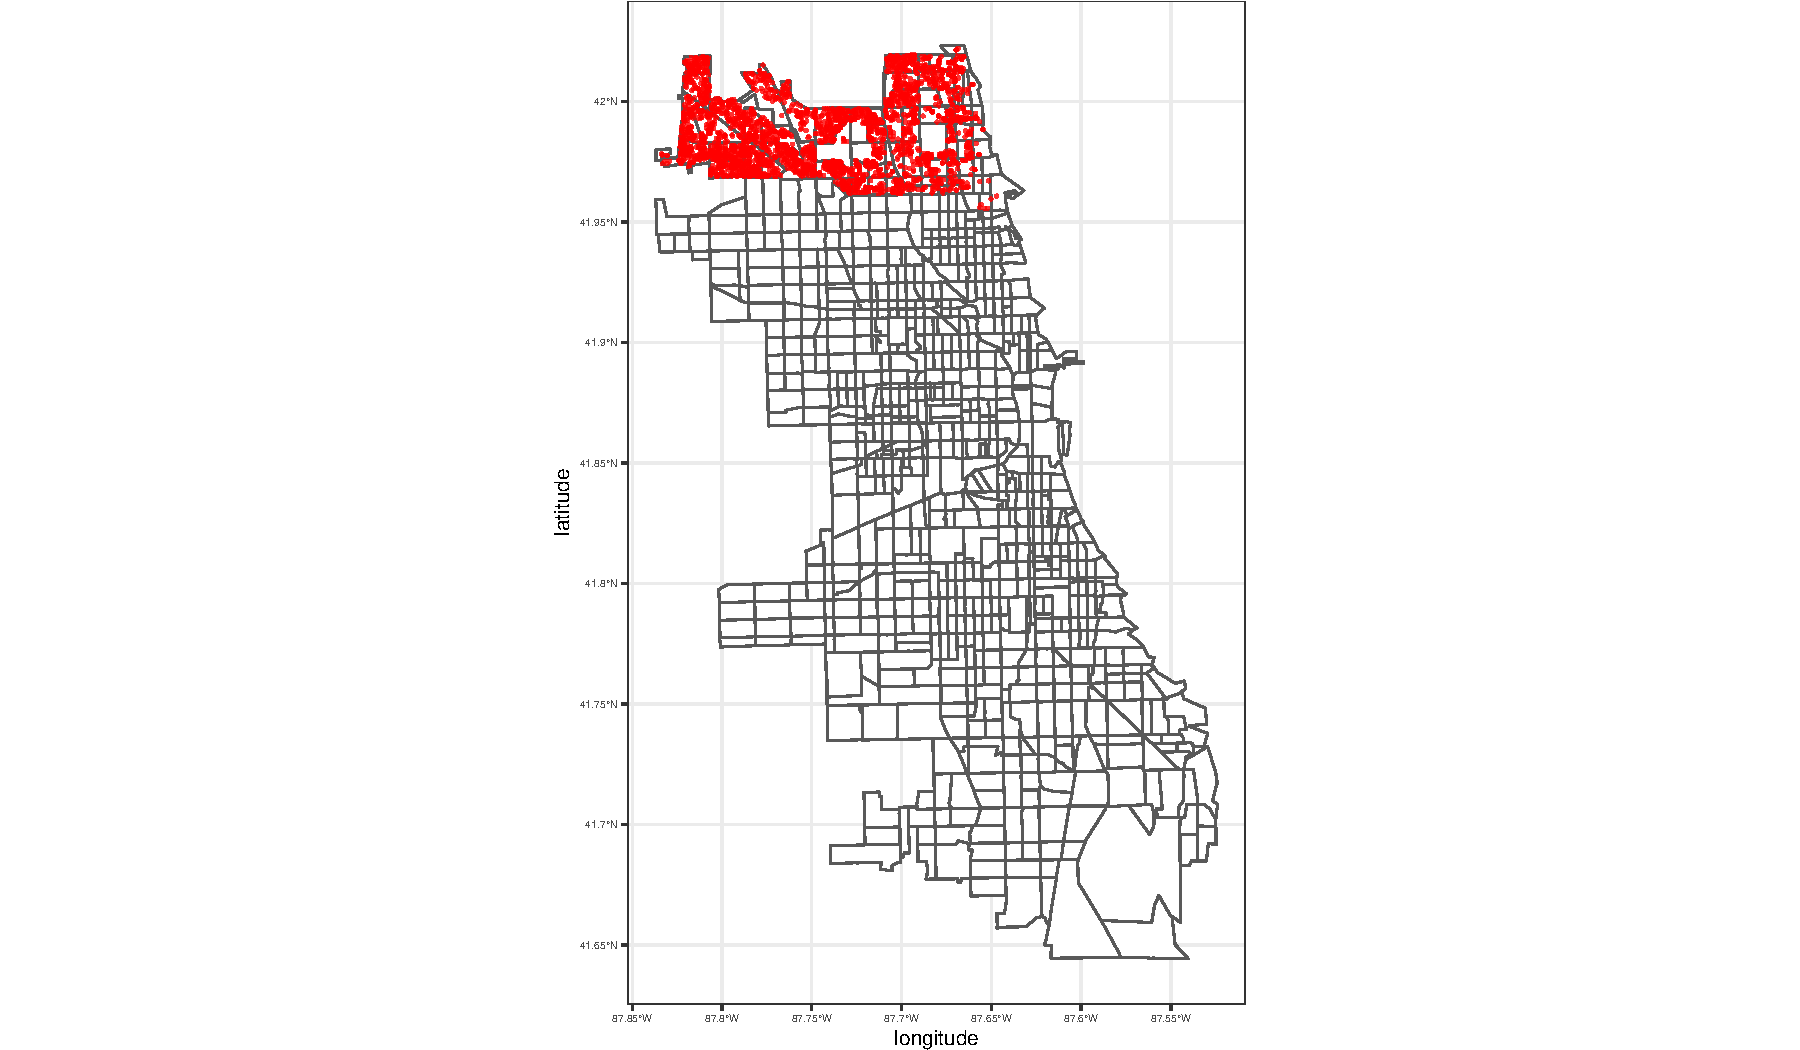
\includegraphics[scale=0.35]{figures/chicago.pdf}
    \end{figure}
    \end{minipage}
\end{frame}
%----------------------------------------------------------------------%
\begin{frame}[fragile]
\frametitle{Example: Predicting House Prices in \texttt{R}}

\begin{itemize}
  \item Train and Test  samples
  \item 30\% / 70\% split
\end{itemize}

\begin{Shaded}
\footnotesize
\begin{Highlighting}[]
\KeywordTok{set.seed}\NormalTok{(}\DecValTok{101010}\NormalTok{) }\CommentTok{\#sets a seed }
\NormalTok{matchdata \textless{}{-}}\StringTok{ }\NormalTok{matchdata }\OperatorTok{\%\textgreater{}\%}\StringTok{ }
\StringTok{                      }\KeywordTok{mutate}\NormalTok{(}\DataTypeTok{price=}\KeywordTok{exp}\NormalTok{(lnprice), }
                             \CommentTok{\#transforms log prices to standard prices}
                             \DataTypeTok{holdout=} \KeywordTok{as.logical}\NormalTok{(}\DecValTok{1}\OperatorTok{:}\KeywordTok{nrow}\NormalTok{(matchdata) }
                             \OperatorTok{\%in\%}\StringTok{ }\KeywordTok{sample}\NormalTok{(}
                             \KeywordTok{nrow}\NormalTok{(matchdata), }\KeywordTok{nrow}\NormalTok{(matchdata)}\OperatorTok{*}\NormalTok{.}\DecValTok{7}\NormalTok{)) }
                             \CommentTok{\#generates a logical indicator 
                             to divide between train and test set}
\NormalTok{                             ) }

\NormalTok{test\textless{}{-}matchdata[matchdata}\OperatorTok{$}\NormalTok{holdout}\OperatorTok{==}\NormalTok{T,]}
\NormalTok{train\textless{}{-}matchdata[matchdata}\OperatorTok{$}\NormalTok{holdout}\OperatorTok{==}\NormalTok{F,]}
\end{Highlighting}
\end{Shaded}

\end{frame}
%----------------------------------------------------------------------%
\begin{frame}[fragile]
\frametitle{Example: Predicting House Prices in \texttt{R}}

\begin{itemize}
 \item Naive approach: model with no covariates, just a constant
 \item $y = \beta_0 + u$
\end{itemize}

\begin{Shaded}
\footnotesize
\begin{Highlighting}[]

\NormalTok{model1\textless{}{-}}\KeywordTok{lm}\NormalTok{(price}\OperatorTok{\textasciitilde{}}\DecValTok{1}\NormalTok{,}\DataTypeTok{data=}\NormalTok{train)}
\KeywordTok{summary}\NormalTok{(model1)}
\end{Highlighting}
\end{Shaded}

\begin{tiny}
\begin{verbatim}

## 
## Call:
## lm(formula = price ~ 1, data = train)
## 
## Residuals:
##     Min      1Q  Median      3Q     Max 
## -258018 -127093  -24018   92732  598482 
## 
## Coefficients:
##             Estimate Std. Error t value Pr(>|t|)    
## (Intercept)   284018       4782   59.39   <2e-16 ***
## ---
## Signif. codes:  0 '***' 0.001 '**' 0.01 '*' 0.05 '.' 0.1 ' ' 1
## 
## Residual standard error: 148300 on 961 degrees of freedom
\end{verbatim}
\end{tiny}

\end{frame}

%----------------------------------------------------------------------%
\begin{frame}[fragile]
\frametitle{Example: Predicting House Prices in \texttt{R}}

In this case our prediction for the log price is the average train
sample average

\[
\hat{y}=\hat{\beta_0}=\frac{\sum y_i}{n}=m
\]

\begin{Shaded}
\footnotesize
\begin{Highlighting}[]
\KeywordTok{coef}\NormalTok{(model1)}
\end{Highlighting}
\end{Shaded}

\begin{tiny}
\begin{verbatim}
## (Intercept) 
##    284017.6
\end{verbatim}
\end{tiny}

\begin{Shaded}
\footnotesize
\begin{Highlighting}[]
\KeywordTok{mean}\NormalTok{(train}\OperatorTok{$}\NormalTok{price)}
\end{Highlighting}
\end{Shaded}

\begin{tiny}
\begin{verbatim}
## [1] 284017.6
\end{verbatim}
\end{tiny}

\end{frame}
%----------------------------------------------------------------------%

\begin{frame}[fragile]
\frametitle{Example: Predicting House Prices in \texttt{R}}

\begin{itemize}
  \item But we are concerned on predicting well our of sample,:
\end{itemize}
\bigskip
\begin{Shaded}
\footnotesize
\begin{Highlighting}[]
\NormalTok{test}\OperatorTok{$}\NormalTok{model1\textless{}{-}}\KeywordTok{predict}\NormalTok{(model1,}\DataTypeTok{newdata =}\NormalTok{ test)}
\KeywordTok{with}\NormalTok{(test,}\KeywordTok{mean}\NormalTok{((price}\OperatorTok{{-}}\NormalTok{model1)}\OperatorTok{\^{}}\DecValTok{2}\NormalTok{))}
\end{Highlighting}
\end{Shaded}

\begin{tiny}
\begin{verbatim}
## [1] 21935777917
\end{verbatim}
\end{tiny}

\begin{itemize}
  \item $\hat AErr(\hat y)=\frac{\sum((y-\hat{y})^2)}{n}=$ \ensuremath{2.1935778\times 10^{10}}
  \item This is our starting point, Can we improve it?
\end{itemize}
  
\end{frame}

%----------------------------------------------------------------------%

\begin{frame}[fragile]
\frametitle{Example: Predicting House Prices in \texttt{R}}

\begin{itemize}
 \item How to improve it?
   \begin{itemize}
   \item One way is using econ theory as guide
   \item hedonic house price function derived directly from the Rosen's theory of hedonic pricing
   \item however, the theory says little on what are the relevant attributes of the house.
   \item So we are going to explore the effects of adding house characteristics on our out $AErr(\hat y)$
  \end{itemize}
  \item The simple inclusion of a single covariate can improve with respect to the \textit{naive} constant only model.
\end{itemize}



\begin{Shaded}
\footnotesize
\begin{Highlighting}[]
\NormalTok{model2\textless{}{-}}\KeywordTok{lm}\NormalTok{(price}\OperatorTok{\textasciitilde{}}\NormalTok{bedrooms,}\DataTypeTok{data=}\NormalTok{train)}
\NormalTok{test}\OperatorTok{$}\NormalTok{model2\textless{}{-}}\KeywordTok{predict}\NormalTok{(model2,}\DataTypeTok{newdata =}\NormalTok{ test)}
\KeywordTok{with}\NormalTok{(test,}\KeywordTok{mean}\NormalTok{((price}\OperatorTok{{-}}\NormalTok{model2)}\OperatorTok{\^{}}\DecValTok{2}\NormalTok{))}
\end{Highlighting}
\end{Shaded}

\begin{tiny}
\begin{verbatim}
## [1] 21695551442
\end{verbatim}
\end{tiny}
\end{frame}


%----------------------------------------------------------------------%

\begin{frame}[fragile]
\frametitle{Example: Predicting House Prices in \texttt{R}}

\begin{itemize}
\item What about if we include more variables?
\end{itemize}

\begin{Shaded}
\footnotesize
\begin{Highlighting}[]
\NormalTok{model3\textless{}{-}}\KeywordTok{lm}\NormalTok{(price}\OperatorTok{\textasciitilde{}}\NormalTok{bedrooms}\OperatorTok{+}\NormalTok{bathrooms}\OperatorTok{+}\NormalTok{centair}\OperatorTok{+}\NormalTok{fireplace}\OperatorTok{+}\NormalTok{brick,}\DataTypeTok{data=}\NormalTok{train)}
\NormalTok{test}\OperatorTok{$}\NormalTok{model3\textless{}{-}}\KeywordTok{predict}\NormalTok{(model3,}\DataTypeTok{newdata =}\NormalTok{ test)}
\KeywordTok{with}\NormalTok{(test,}\KeywordTok{mean}\NormalTok{((price}\OperatorTok{{-}}\NormalTok{model3)}\OperatorTok{\^{}}\DecValTok{2}\NormalTok{))}
\end{Highlighting}
\end{Shaded}

\begin{tiny}
\begin{verbatim}
## [1] 21111169595
\end{verbatim}
\end{tiny}


\begin{itemize}
\item Note that the $AErr$ is once more reduced. If we include all?
\end{itemize}



\begin{Shaded}
\footnotesize
\begin{Highlighting}[]
\NormalTok{model4\textless{}{-}}\KeywordTok{lm}\NormalTok{(price}\OperatorTok{\textasciitilde{}}\NormalTok{bedrooms}\OperatorTok{+}\NormalTok{bathrooms}\OperatorTok{+}\NormalTok{centair}\OperatorTok{+}\NormalTok{fireplace}\OperatorTok{+}\NormalTok{brick}\OperatorTok{+}
\StringTok{                }\NormalTok{lnland}\OperatorTok{+}\NormalTok{lnbldg}\OperatorTok{+}\NormalTok{rooms}\OperatorTok{+}\NormalTok{garage1}\OperatorTok{+}\NormalTok{garage2}\OperatorTok{+}\NormalTok{dcbd}\OperatorTok{+}\NormalTok{rr}\OperatorTok{+}
\StringTok{                }\NormalTok{yrbuilt}\OperatorTok{+}\KeywordTok{factor}\NormalTok{(carea)}\OperatorTok{+}\NormalTok{latitude}\OperatorTok{+}\NormalTok{longitude,}\DataTypeTok{data=}\NormalTok{train)}
\NormalTok{test}\OperatorTok{$}\NormalTok{model4\textless{}{-}}\KeywordTok{predict}\NormalTok{(model4,}\DataTypeTok{newdata =}\NormalTok{ test)}
\KeywordTok{with}\NormalTok{(test,}\KeywordTok{mean}\NormalTok{((price}\OperatorTok{{-}}\NormalTok{model4)}\OperatorTok{\^{}}\DecValTok{2}\NormalTok{))}
\end{Highlighting}
\end{Shaded}

\begin{tiny}
\begin{verbatim}
## [1] 20191829518
\end{verbatim}
\end{tiny}

\begin{itemize}
  \item Is there a limit to this improvement? Can we keep adding features and complexity?
\end{itemize}

\end{frame}

%----------------------------------------------------------------------%
\begin{frame}[fragile]
\frametitle{Example: Predicting House Prices in \texttt{R}}

\begin{itemize}
  \item Is there a limit to this improvement? Can we keep adding features and complexity?
  \item Let's try a bunch of models
\end{itemize}

\begin{Shaded}
\scriptsize
\begin{Highlighting}[]
\NormalTok{model5\textless{}{-}}\KeywordTok{lm}\NormalTok{(price}\OperatorTok{\textasciitilde{}}\KeywordTok{poly}\NormalTok{(bedrooms,}\DecValTok{2}\NormalTok{)}\OperatorTok{+}\KeywordTok{poly}\NormalTok{(bathrooms,}\DecValTok{2}\NormalTok{)}\OperatorTok{+}
\StringTok{                }\NormalTok{centair}\OperatorTok{+}\NormalTok{fireplace}\OperatorTok{+}\NormalTok{brick}\OperatorTok{+}
\StringTok{                }\NormalTok{lnland}\OperatorTok{+}\NormalTok{lnbldg}\OperatorTok{+}\NormalTok{rooms}\OperatorTok{+}
\StringTok{                }\NormalTok{garage1}\OperatorTok{+}\NormalTok{garage2}\OperatorTok{+}\NormalTok{dcbd}\OperatorTok{+}\NormalTok{rr}\OperatorTok{+}
\StringTok{                }\NormalTok{yrbuilt}\OperatorTok{+}\KeywordTok{factor}\NormalTok{(carea)}\OperatorTok{+}\KeywordTok{poly}\NormalTok{(latitude,}\DecValTok{2}\NormalTok{)}\OperatorTok{+}
\StringTok{                }\KeywordTok{poly}\NormalTok{(longitude,}\DecValTok{2}\NormalTok{),}\DataTypeTok{data=}\NormalTok{train)}
\NormalTok{test}\OperatorTok{$}\NormalTok{model5\textless{}{-}}\KeywordTok{predict}\NormalTok{(model5,}\DataTypeTok{newdata =}\NormalTok{ test)}

\NormalTok{model6\textless{}{-}}\KeywordTok{lm}\NormalTok{(price}\OperatorTok{\textasciitilde{}}\KeywordTok{poly}\NormalTok{(bedrooms,}\DecValTok{2}\NormalTok{)}\OperatorTok{+}\KeywordTok{poly}\NormalTok{(bathrooms,}\DecValTok{2}\NormalTok{)}\OperatorTok{+}\NormalTok{centair}\OperatorTok{+}\NormalTok{fireplace}\OperatorTok{+}\NormalTok{brick}\OperatorTok{+}
\StringTok{                }\NormalTok{lnland}\OperatorTok{+}\NormalTok{lnbldg}\OperatorTok{+}\NormalTok{garage1}\OperatorTok{+}\NormalTok{garage2}\OperatorTok{+}\NormalTok{rr}\OperatorTok{+}
\StringTok{                }\NormalTok{yrbuilt}\OperatorTok{+}\KeywordTok{factor}\NormalTok{(carea)}\OperatorTok{+}\KeywordTok{poly}\NormalTok{(latitude,}\DecValTok{2}\NormalTok{)}\OperatorTok{+}\KeywordTok{poly}\NormalTok{(longitude,}\DecValTok{2}\NormalTok{),}
\StringTok{                }\DataTypeTok{data=}\NormalTok{train)}
\NormalTok{test}\OperatorTok{$}\NormalTok{model6\textless{}{-}}\KeywordTok{predict}\NormalTok{(model6,}\DataTypeTok{newdata =}\NormalTok{ test)}

\NormalTok{model7\textless{}{-}}\KeywordTok{lm}\NormalTok{(price}\OperatorTok{\textasciitilde{}}\KeywordTok{poly}\NormalTok{(bedrooms,}\DecValTok{2}\NormalTok{)}\OperatorTok{+}\KeywordTok{poly}\NormalTok{(bathrooms,}\DecValTok{2}\NormalTok{)}\OperatorTok{+}\NormalTok{centair}\OperatorTok{+}\NormalTok{fireplace}\OperatorTok{+}\NormalTok{brick}\OperatorTok{+}
\StringTok{                }\NormalTok{lnland}\OperatorTok{+}\NormalTok{lnbldg}\OperatorTok{+}\NormalTok{garage1}\OperatorTok{+}\NormalTok{garage2}\OperatorTok{+}\NormalTok{rr}\OperatorTok{+}
\StringTok{                }\NormalTok{yrbuilt}\OperatorTok{+}\KeywordTok{factor}\NormalTok{(carea)}\OperatorTok{+}\KeywordTok{poly}\NormalTok{(latitude,}\DecValTok{3}\NormalTok{)}\OperatorTok{+}\KeywordTok{poly}\NormalTok{(longitude,}\DecValTok{3}\NormalTok{),}
\StringTok{                }\DataTypeTok{data=}\NormalTok{train)}
\NormalTok{test}\OperatorTok{$}\NormalTok{model7\textless{}{-}}\KeywordTok{predict}\NormalTok{(model7,}\DataTypeTok{newdata =}\NormalTok{ test)}
\end{Highlighting}
\end{Shaded}


\end{frame}
%----------------------------------------------------------------------%
\begin{frame}[fragile]
\frametitle{Example: Predicting House Prices in \texttt{R}}

   \begin{figure}[H] \centering
            \captionsetup{justification=centering}  
            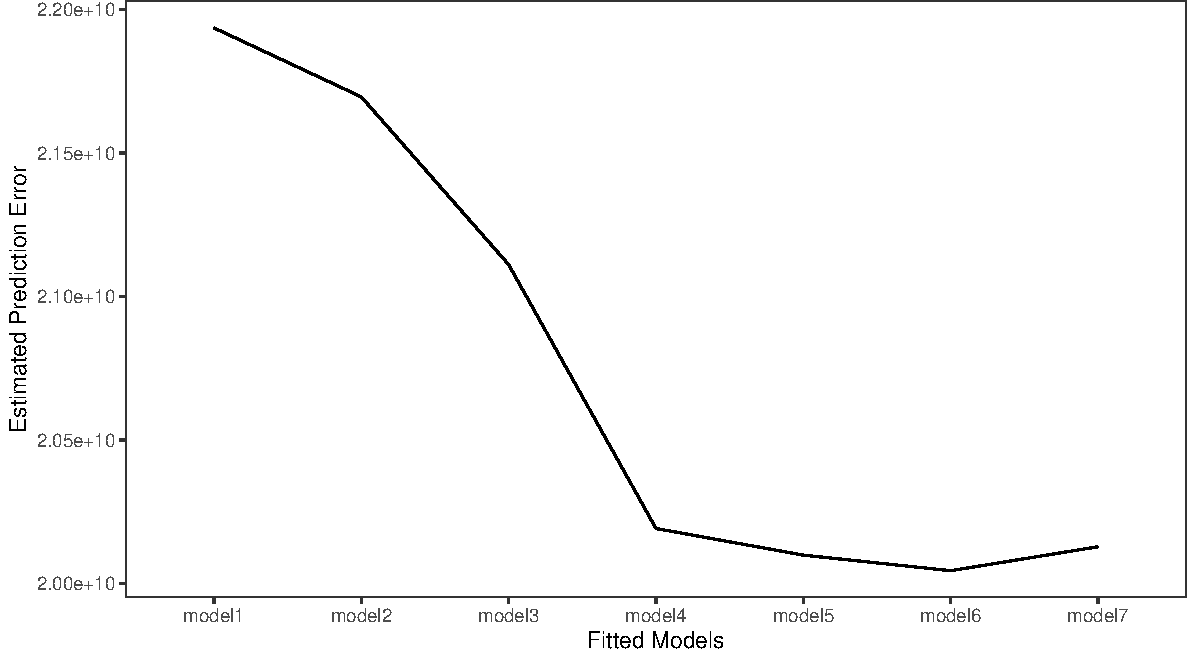
\includegraphics[scale=.4]{figures/mse_plot_ch3-1.pdf}
    \end{figure}

\end{frame}
%----------------------------------------------------------------------%
\begin{frame}[fragile]


\begin{itemize}
  \item Take aways from the example
  \bigskip
  \item Classical econometrics set up, choosing between smaller and larger models
  \bigskip
  \item More complexity, the prediction error keeps getting smaller.
  \bigskip
  \item The choice of a model's complexity faces a bias/variance trade-off.  
  \bigskip
  \item Open question: how to find the optimal complexity level? \\ {\tiny (later on the course)}

\end{itemize}


\end{frame}

%----------------------------------------------------------------------%
%----------------------------------------------------------------------%
\section{Review}
%----------------------------------------------------------------------%
\begin{frame}
\frametitle{Review \& Next Steps}
  
  \begin{itemize} 
    \item Linear Regression
    \item Prediction vs Estimation
    \item Train and Test Samples
    \item Example in \texttt{R}
  \bigskip  

  
  \item  {\bf Next Class:} Big Data intro, OLS Numerical Properties Computation.
  \bigskip
  \item Questions? Questions about software? 
  
  \end{itemize}


\end{frame}

%----------------------------------------------------------------------%

\section{Further Readings}
%----------------------------------------------------------------------%
\begin{frame}
\frametitle{Further Readings}

\begin{itemize}
  \item Davidson, R., \& MacKinnon, J. G. (2004). Econometric theory and methods (Vol. 5). New York: Oxford University Press.
  \bigskip
  \item James, G., Witten, D., Hastie, T., \& Tibshirani, R. (2013). An introduction to statistical learning (Vol. 112, p. 18). New York: springer.
  \bigskip
  \item Friedman, J., Hastie, T., \& Tibshirani, R. (2001). The elements of statistical learning (Vol. 1, No. 10). New York: Springer series in statistics.
  \bigskip
  \item Murphy, K. P. (2012). Machine learning: a probabilistic perspective. MIT press.

\end{itemize}

\end{frame}


\end{document}


